\documentclass[12pt]{article}
\usepackage{fullpage,amsmath}% mathtools}
\usepackage{setspace}
\usepackage{graphicx, psfrag, amsfonts}
\usepackage{natbib}
\usepackage{amsthm}
\usepackage{multirow}
\usepackage{hhline}
%\usepackage{color}
\usepackage[position=t,singlelinecheck=off]{subcaption}
\usepackage{caption, setspace}
%\usepackage[position=t,singlelinecheck=off]{subfigure}
 \pdfminorversion=4

\def\bgam{\mbox{\boldmath $\gamma$}}
\def\bth{\mbox{\boldmath $\theta$}}
\def\bbeta{\mbox{\boldmath $\beta$}}
\def\blam{\mbox{\boldmath $\lambda$}}
\def\bmu{\mbox{\boldmath $\mu$}}

\newcommand{\bx}{\mbox{\boldmath $x$}}
\newcommand{\bu}{\mbox{\boldmath $u$}}
\newcommand{\bc}{\�mbox{\boldmath $c$}}
\newcommand{\bs}{\mbox{\boldmath $s$}}
\newcommand{\by}{\mbox{\boldmath $y$}}
\newcommand{\bz}{\mbox{\boldmath $z$}}
\newcommand{\bv}{\mbox{\boldmath $v$}}
\newcommand{\bb}{\mbox{\boldmath $b$}}
\newcommand{\bzero}{\mbox{\boldmath $0$}}
\newcommand{\thstarj}{\mbox{$\theta^\star_j$}}
\newcommand{\bths}{\mbox{$\btheta^\star$}}
\newcommand{\pkg}[1]{{\fontseries{b}\selectfont #1}} 

\newcommand{\ud}{\mathrm{d}}
\newcommand{\uI}{\mathrm{I}}
\newcommand{\uP}{\mathrm{P}}
\newcommand{\up}{\mathrm{p}}
\newcommand{\mb}{\mathbf}
\newcommand{\mc}{\mathcal}




\newcommand{\Bern}{\mbox{Bern}}
\newcommand{\Nor}{\mbox{N}}
\newcommand{\Ga}{\mbox{Gamma}}
\newcommand{\Dir}{\mbox{Dir}}
\newcommand{\Ber}{\mbox{Ber}}
\newcommand{\Be}{\mbox{Be}}
\newcommand{\Unif}{\mbox{Unif}}
\newcommand{\Binom}{\mbox{Bin}}
\newcommand{\IG}{\mbox{IG}}

\newcommand{\Xs}{X^\star}
\newcommand{\Lc}{{\cal L}}


\usepackage[dvipsnames,usenames]{color}
\newcommand{\yy}{\color{magenta}\it}
\newcommand{\jj}{\color{Black}\rm}
\newcommand{\yjnote}[1]{\footnote{\color{Brown}\rm #1 \color{Black}}}
\newtheorem{theorem}{Theorem}[section]
\newtheorem{definition}[theorem]{\bf Definition}
\newtheorem{lemma}[theorem]{\bf Lemma}
\newtheorem{corollary}[theorem]{\bf Corollary}
\newtheorem{proposition}[theorem]{\bf Proposition}
\newtheorem{assumption}[theorem]{\bf Assumption}
\newtheorem{example}[theorem]{\bf Example}
\newtheorem{remark}[theorem]{\bf Remark}


\newcommand{\iid}{\stackrel{iid}{\sim}}
\newcommand{\indep}{\stackrel{indep}{\sim}}

\doublespacing
\setlength{\textwidth}{6 in}

% commands for for editing
\usepackage{color}
\newcommand{\red}[1]{{\color{red}#1}}
\newcommand{\blue}[1]{{\color{blue}#1}}
\newcommand{\brown}[1]{{\color{brown}#1}}
\newcommand{\green}[1]{{\color{green}#1}}
\newcommand{\magenta}[1]{{\color{magenta}#1}}
\DeclareMathOperator*{\argmin}{\arg\!\min}
\graphicspath{{figures/}}


\makeatletter
\newcommand{\labitem}[2]{%
\def\@itemlabel{\textbf{#1}{.}}
\item
\def\@currentlabel{#1}\label{#2}}
\makeatother


%  Points to handle in preparing the manuscript
%
%  1.  Out of sample evaluation of the model.  We should go with trimmed mean log-likelihood (trimming the cases
%       that contribute least to log-likelihood).  Justification for the trimming mentioned in a sentence
%       here, to be more carefully and completely done in separate work (with Yoonsuh).  
%
%  3.  Add quite a number of references to Section 2.  This is where we should catch the old work
%      that conditions on the sample mean and proceeds through asymptotic approximation, Peter 
%      Hoff's work on ranks, Holmes and Walker's work, and ABC.  New text needs to accompany the
%      references, making clear what the other work does and how ours differs.  The new text should
%      be quite brief.  
%
%  4.  A big question.  Should we try to add any asymptotic theory?  A Section 3.4?  See next comment.  
%      My vote is "no".  
%
%  5.  Page limitations.  A goal for the entire manuscript is 30 pages.  Current length is 34+, spilling
%      onto page 35.  But, additions will include the abstract (1/2 page or so), conclusions (1 page or 
%      so), more references (another half page?), and more writing scattered throughout.  Redoing
%      figures (two to drop) and tables will save a modest amount of space.   I propose that we 
%      hold off on adding new content until we see how long the paper is.  Also, new content along
%      the lines of point 4 would mean that we have to prove/use existing results to show the truth
%      of whatever we claim!  
%
%  6.  Confirm with Nationwide that they are okay with our using their data and that they are comfortable
%       with the descriptions we have in the paper.  
%
%  7.  Fit the hierarchical model, conditioning on the robust summaries at each leaf in the model.  
%
%  9.  A hedge on computations?  There are examples (pathological in some senses) for which a basic
%      MCMC based on the complete data works, but where conditioning on a poorly chosen T(y) leads
%      to a reducible Markov chain.  I don't think this happens when the support of y is the same for all
%      \theta (it may be that mutual absolute continuity of all distributions for y|\theta is needed, though
%      definitions of "support" vary somewhat).  I think we can ignore this here, but an example could go
%      into the dissertation.  (one sentence now included to hint at this).  



%  To be added
%
%  1.  Abstract.  
%
%  2.  Conclusions.  To be written later.  I will take a pass at them once a few results are filled in for
%       the data analysis.  
%

%  John.  
%  See notes in red throughout.  The overarching goal is to move the manuscript toward completion.  
%  To do so means filling in details to get them taken care of.  Big batches are (i) references, (ii) 
%  deciding on notation for the estimator (b to replace beta?), (iii) verifying that the theorems have the
%  right conditions, (iv) patching figures, (v) adding material for the examples, and (vi) deciding whether
%  the figure and text on the last two pages is needed.  
%  If you want to add comments for us, pick a color other than red and add them in that color.  

%  Yoon.  
%  A check on the theorems would be great.  No need, I think, to dig out the paper by Miao and Ben Israel
%  as that part of the math is fine (I'll check to make sure that all conditions for our use of the theorems have
%  been stated in the Corollary).  Once more details are in place, proof reading and adjustment.  

%\newpage
\title{Bayesian Restricted Likelihood Methods}
\author{John R. Lewis, Steven N. MacEachern and  Yoonkyung Lee \\
{\small \it Department of Statistics, The Ohio State University, Columbus, Ohio 43210}\\
{\small lewis.865@osu.edu, snm@stat.osu.edu and yklee@stat.osu.edu}
\thanks{This research has been supported by Nationwide Insurance Company and by the NSF under grant numbers DMS-1007682 and DMS-1209194.  The views in this paper are not necessarily those of Nationwide Insurance or the NSF.}} 
\begin{document}
\date{}
\maketitle

\begin{abstract}
Bayesian methods have proven themselves to be successful across a wide
range of scientific problems and have many well-documented advantages
over competing methods. However, these methods run into difficulties
for two major and prevalent classes of problems: handling data sets
with outliers and dealing with model misspecification. We outline the
drawbacks of previous solutions to both of these problems (e.g., use of
heavy-tailed likelihoods) and propose the restricted likelihood as an
alternative.  When working with restricted likelihood, we summarize
the data through a set of (insufficient) statistics,
targeting inferential quantities of interest, and update the prior
distribution with the summary statistics rather than the complete
data.  By choice of conditioning statistics, we
retain the main benefits of Bayesian methods while reducing the
sensitivity of the analysis to features of the data not picked up by
the conditioning statistics. A major
contribution is the development of a data augmented MCMC algorithm
for the linear model and a wide range of choices for
summary statistics. We demonstrate the method on an
insurance agency data set containing many outliers and subject to model
misspecification. Success is manifested in better predictive
performance for data points of interest as compared to competing
methods.

\noindent KEYWORDS: Approximate Bayesian computation, Markov chain
Monte Carlo, M-estimation, Robust regression.


\end{abstract}

\section{Introduction}

Bayesian methods have provided successful solutions to a wide range of scientific problems, with their value
having been demonstrated both empirically and theoretically.  
In simple settings, the success of the methods is often attributed to formal optimality properties, sometimes derived
through the laws of subjective probability 
and sometimes through admissibility and the complete class
theorems of decision theory.  In complex settings, the hierarchical model allows one to create 
and fit sophisticated models that may, for example, pool information across similar problems.  

The development of Bayesian inference relies on a complete Bayesian model consisting of 
three elements:  the prior distribution, the loss function, and the likelihood or sampling density.  While formal
optimality of Bayesian methods is unquestioned if one accepts the validity of all three of these elements, 
 a healthy skepticism encourages us to question each of them.  Concern about the prior distribution has
been addressed through the development of techniques for subjective elicitation \citep{garthwaite2005} and
the rise of objective Bayesian methods \citep{berger2006}.  
Concern about the loss function is reflected in, for example, the
extensive literature on Bayesian hypothesis tests \citep{kass1995}.  
The sampling density has been given less attention from a specifically
Bayesian view, although the work on predictive diagnostics \citep{box1980} departs from classical
traditions.  

The focus of this work is the intersection of Bayesian methodology and data analysis.  In particular, 
we develop techniques to handle imperfections in the sampling density.  These imperfections often show
themselves through the presence of outliers--here taken to be cases not reflecting the phenomenon under
study--in the data set.  
There are three main solutions to Bayesian outlier-handling.  The first is to replace the basic sampling
density with a mixture model which includes one component for the ``good'' data and a second 
component for the ``bad'' data.  With this approach, the prior distribution is updated with the likelihood
from the mixture model to obtain the complete-data posterior distribution.  The good component of
the sampling density is used for prediction of future good data.  The second approach replaces the
basic sampling density with a thick-tailed density in an attempt to discount outliers, yielding techniques that 
often provide solid estimates of the center of the distribution but 
do not easily translate to predictive
densities for further good data.  The third approach fits a flexible (typically nonparametric) model to 
the data, producing a Bayesian version of a density estimate for both good and bad data.  In recent 
development, inference 
is made through the use of robust inference functions \citep[][in press]{lee2013}.  

The traditional strategies for handling outliers all have their drawbacks.  While we view the sampling 
density for the good data as stable, the outlier-generating processes 
may be transitory in nature, constantly shifting as the source of bad data changes.  This prevents
us from appealing to large-sample arguments to claim that, with enough data, we can nail down a
model for both good and bad data combined.  Instead of attempting to model both good and bad
data, we propose a novel strategy for handling outliers:  the use of restricted likelihood.  In a nutshell,
we begin with a complete model   
as if all of the data are good.
But rather than driving the move from prior distribution to posterior
distribution by the entire likelihood, we use only the likelihood of a
few summary statistics which typically target inferential quantities
of interest.  We call this reduced likelihood a restricted likelihood.  The 
update is a formal update from prior distribution to posterior distribution, based on the sampling density
of the summary statistics. 
 In our approach, the reader will identify a stream of reasoning which is manifested in
classical M-estimation, generalized estimating equations, approximate Bayesian computation,
and elsewhere.  The novelty of the work is twofold.  We make use of
classical robust estimators as  summary statistics in a formal
Bayesian framework, using the sampling density of the estimators as a replacement for the 
sampling density of the data.  We advance the argument that conditioning on an insufficient
summary of the data is sound practice, rather than merely being done for computational and 
modelling convenience.  

In addition to outlier-prone data, the sampling density can err due to model misspecification.  
The traditional view is that, if the model is inadequate, one should build a better model.  In our
empirical work, as data sets have become larger and more complex, we have bumped into 
settings where we cannot realistically build the perfect model.  We ask the question ``by attempting
to improve our model through elaboration, will the overall performance of the model suffer?''  If yes,
we avoid the elaboration, retaining a model with some level of misspecification.  Acknowledging that
the model is misspecified implies acknowledging that the sampling density is incorrect, exactly as
we do when outliers are present.  In this sense, misspecified models and outliers are reflections of the
same phenomenon, and we recommend a common solution for dealing with the problem.  

The remainder of the paper develops Bayesian restricted likelihood (Section~\ref{restrictedlikelihood}), shows
how it can be applied to a Bayesian linear model (Section~\ref{BayesLinMod}), illustrates its use
on an insurance agencies data set with a novel twist on model evaluation (Section~\ref{Applications}), 
and wraps up with a discussion (Section~\ref{Conclusions}).  
A major contribution of this work is the computational strategy whose legitimacy is established 
in Section~\ref{BayesLinMod}.  The technical proofs are in the appendix.   

\section{Restricted Likelihood}
\label{restrictedlikelihood}

To describe the use of restricted likelihood in a Bayesian framework, 
we begin with a pair of simple examples
for the one-sample problem.  In each, the model takes the
data $\by=(y_1,\ldots,y_n)$
to be a random sample
of size $n$ from a continuous distribution indexed by a parameter vector $\bth$.  The standard, or complete,
likelihood would be $L(\bth | \by) = \prod_{i=1}^n f(y_i | \bth)$.  

As a first example, we consider the case where a subset of the data are known to be 
bad in the sense of not
  informing us about $\bth$--and where the subset is known.  This case mimics the setting where outliers in
a data set are identified and discarded before a formal analysis is done.  
Without loss of generality, we label the good 
cases $1$ through $n-k$ and the bad 
cases $n-k+1$ through $n$.  
The relevant likelihood to be used to move from prior distribution to posterior distribution is clearly 
$L(\bth | y_1, \ldots, y_{n-k}) = \prod_{i=1}^{n-k} f(y_i | \bth)$.  
For an equivalent analysis, we rewrite the entire likelihood as the product of two pieces,
\begin{eqnarray}
\label{OutlyingCases}
L(\bth | \by)  
= \left( \prod_{i=1}^{n-k} f(y_i | \bth) \right) \left( \prod_{i=n-k+1}^{n} f(y_i | \bth) \right) ,
\end{eqnarray}
where the second term may not actually involve $\bth$.
We wish to keep the first piece and drop the second for better inference on $\bth$.

A second example involves deliberate censoring of small and large observations.  This is
sometimes done as a precursor to the analysis of reaction time experiments (e.g., \cite{ratcliff1993}).  
With lower
and upper censoring times at $t_1$ and $t_2$, the post-censoring sampling distribution
is of mixed form, with masses $F(t_1|\bth)$ at $t_1$ and $1-F(t_2|\bth)$ at $t_2$,
and density $f(y | \bth)$ for $y \in (t_1, t_2)$.  We adjust the original data $y_i$,
producing $x_i$ by defining $x_i = t_1$ if $y_i \leq t_1$, 
$x_i = t_2$ if $y_i \geq t_2$, and $x_{i}=y_{i}$ otherwise.  
The adjusted update is performed with $L(\bth | \bx)$. 
With slightly non-standard notation, we let $g(t_1|\bth) = F(t_1|\bth)$,
$g(t_2 | \bth) = 1 - F(t_2|\bth)$, and $g(y|\bth)=f(y|\bth)$ for
$y \in (t_1, t_2)$.
Alternatively, we may rewrite the entire likelihood as the product of
two pieces, 
\begin{eqnarray}
\label{Censoring}
L(\bth | \by) =  
\left( \prod_{i=1}^n g(x_i | \bth) \right) \left( \prod_{i=1}^n f(y_i|x_i,\bth) \right) ,  
\end{eqnarray}
and retain only the first for the formal update.  

Further examples abound.  In a completely randomized experimental design, we randomize %our 
experimental units to treatment conditions and then ignore the details of the observed randomization \citep{dean1999}; 
in work with contingency tables,  
we collapse categories with small counts, coarsening the scale of %our 
data \citep{agresti2002}; in meta-analysis, we ignore the individual patient-level data and instead
work with estimated effects from the studies \citep{orourke2007}.  
Further examples are described in \cite{lewis2014}.  
To describe the approach in (\ref{OutlyingCases}), 
(\ref{Censoring}), and these other settings,
we write the complete data likelihood in two pieces, as indicated below:
\begin{eqnarray}
\label{FullLikelihood}
L(\bth | \by)  
& = & f(T(\by) | \bth) \,\, f(\by | T(\by), \bth) .  
\end{eqnarray}
In the dropped case example, the conditioning statistic is $T(\by) = (y_1, \ldots, y_{n-k})$.  In 
the censoring example, the conditioning statistic is $T(\by) = (x_1, \ldots, x_n)$.  We refer to 
$f(T(\by) | \bth)$ as the restricted likelihood.  

Bayesian methods can make use of restricted likelihood in place of the complete data likelihood
since $T(\by)$ is a well-defined random variable with a probability distribution indexed by $\bth$.  
The update from prior distribution to posterior distribution is 
made on the basis of $f(T(\by)|\bth)$ rather than $f(\by|\bth)$.  This leads to the restricted likelihood posterior 
\begin{eqnarray}
\label{RestrictedPosterior}
\pi(\bth | T(\by)) & = & \frac{\pi(\bth) f(T(\by) | \bth)}{m(T(\by))} ,
\end{eqnarray}
where $m(T(\by))$ is the marginal distribution of $T(\by)$ under the prior distribution.  
Predictive statements for further (good) data rely on the model.  For another observation,
say $y_{n+1}$, we would have the predictive density 
\[
f(y_{n+1} | T(\by)) = \int f(y_{n+1} | \bth) \pi(\bth | T(\by))\ d\bth .  
\]

Direct use of restricted likelihood appears in many areas of the literature.  The motivation is often similar to ours:   
concern about model misspecification.  For example, the use of rank likelihoods is discussed by \cite{savage1969}, \cite{pettitt1983, pettitt1982}, and more recently by \cite{hoff2013}. Asymptotic properties of restricted posteriors are studied by \cite{doksum1990}, \cite{clarke1995}, \cite{yuan2004},  and \cite{hwang2005}. The tenor of these asymptotic 
results is that, for a variety of conditioning statistics with non-trivial regularity conditions on prior, model, and likelihood, the
posterior distribution resembles the asymptotic sampling distribution of the conditioning statistic.  

Restricted likelihoods have also been used as practical approximations to the full likelihood. For example, \cite{pratt1965} appeals to heuristic arguments regarding approximate sufficiency to justify the use of the restricted likelihood of the sample mean and standard deviation. Approximate sufficiency is  often appealed to when applying approximate Bayesian computation (ABC), a collection of posterior approximation methods which has recently experienced success in applications to epidemiology, genetics, and quality control \citep[see, for example,][]{tavare1997, pritchard1999,  marjoram2003, fearnhead2012}. ABC is typically used when likelihoods are intractable but simulation of new data from the model is easily done. In the cited references, interest lies in the full data posterior and ABC is used for computational 
convenience.  Consequently, effort is made to choose a $T(\by)$ such that the likelihood 
$L(\bth|\by) \approx L(\bth|T(\by))$.  Technical limitations of ABC imply that in realistic (and all non-discrete) settings,
the conditioning is not exact, but approximate.  

In a related, but distinctly different, approach which also takes advantage of summary statistics, the full data log likelihood is replaced by a loss function \citep[e.g.][]{bissiri2013} in an effort to concentrate inference only on parameters of interest. In contrast, the restricted likelihood is formulated using a full probability model, allowing for a formal Bayesian update, while remaining robust to misspecification. This work extends the use of restricted likelihood by arguing that its use is sound practice, and also by expanding the class of conditioning statistics in which exact conditioning can be achieved well beyond ranks.  Our methods do not rely on asymptotic properties or approximate conditioning as in previous work (e.g., \cite{albert1988},\cite{hoffwakefield2013}).  

The key to productive use of restricted likelihood is the choice of $T(\by)$ and the development
of computational strategies that allow us to truly condition on the observed $T(\by)$ and 
fit the model in formal Bayesian fashion.  In this work, we focus
on robustness, and natural choices of $T(\by)$ include a set of middling order statistics, a trimmed
mean, or a classical robust estimator of location and/or scale.  
We have previously implemented all of these methods for one-sample problems 
where we have found them to perform well (e.g., \cite{lewis2012}).  Of these versions, the most 
extensible to the linear model are the
M-estimators, 
in the tradition of \cite{huber1964}.  
The computational strategies we devise in subsequent sections allow us to apply Bayesian
restricted likelihood inference well beyond regression models for the mean of a distribution.  In particular, 
quantile regression falls within the framework we develop.
The next section develops the necessary computational
strategies.  


\section{Restricted Likelihood for the Linear Model}
\label{BayesLinMod}

\subsection{The Bayesian linear model}
We focus on the use of restricted likelihood for the Bayesian linear
model with a standard formulation: 
\begin{eqnarray}
\label{LinearModel}
\bbeta & \sim & \pi_1(\bbeta); \qquad \sigma^2  \sim  \pi_2(\sigma^2)
\nonumber\\
y_i  & =  & x_i^\top \bbeta + \epsilon_i , \mbox{ for } i = 1, \ldots, n 
\end{eqnarray}
where $x_i$ and $\bbeta \in \mathbb{R}^p$, 
and the $\epsilon_i$ are independent 
draws from a distribution with center $0$ and scale $\sigma$.
Two conditions are imposed on the model:
\begin{itemize}
\labitem{C1}{fullRank} The $n \times p$ design matrix, $X$, whose $i^{th}$ row is $x_i^\top$, 
is of full column rank.  
\labitem{C2}{supReal} The $\epsilon_i$ are a random sample from some distribution which has a density with 
respect to Lebesgue measure on the real line and for which the support is the real line.  
\end{itemize}
Both conditions can
be relaxed, although this would necessitate restating several later results.  
In the sequel, we specifically consider both normal and $t$ distributions with
mean $0$ and variance $\sigma^2$ for the $\epsilon_i$ 
but note that our methods apply much more widely.  The prior distributions $\pi_1$ and $\pi_2$ can take
many forms and may be joined to form a joint distribution for non-independent $\bbeta$
and $\sigma^2$.  The conditionally conjugate normal/inverse gamma pair is a common 
choice.  

The methods we develop apply to the linear model in (\ref{LinearModel}) and to many variations
on it.  As summary statistics for the data, we consider M-estimators for the 
coefficients in the linear model and an associated 
estimator of the scale.  These estimates convey information about $\bth=(\bbeta,\sigma)$
while downweighting outliers.  The M-estimator of $\bbeta$ is determined by a $\rho$ function through the minimization
\begin{eqnarray}
\bb(X,\by) & = & \argmin_{\bbeta} \sum_{i=1}^n \rho(\frac{y_i - x_i^\top \bbeta}{\sigma}) .  
\end{eqnarray} 
The scale estimator $s(X,\by)$ is determined simultaneously as another M-estimator or is determined through
a separate calculation, for example the mean-absolute-deviation from an $\ell_1$ regression fit. 
Continuity of the distribution of the $\epsilon_i$ is important as it translates into a continuous distribution for $\bb$, 
which is presumed for our computational strategy.  The results we derive also apply to estimators that are
not M-estimators.  

\subsection{Computational strategy}
\label{highDim}
For low-dimensional statistics $T(\by)$ and $\bth$, the direct computational strategies described in \cite{lewis2012} can be used
to evaluate the restricted likelihood posterior.  
These strategies rely on generation of complete data sets from different values of $\bth$.  
Each complete data set leads to a statistic $T(\by|\bth)$, and these generated statistics are used to estimate the
density at $T(\by_{obs}|\bth)$
which is then fed into Bayes theorem for the update from prior distribution to posterior distribution.  
A variety of  variance reduction techniques which exploit 
properties of the distribution of $\by$ 
improve the performance of these strategies.  

For high-dimensional statistics $T(\by)$ or high-dimensional parameters $\bth$, direct computational 
strategies break down.  When the conditioning statistic is of high-dimension, density estimation becomes 
difficult and the associated approximate update in (\ref{RestrictedPosterior}) is unstable; when $\bth$
is high dimensional, grid-based calculation and other numerical integration strategies fail.  However, Markov 
chain Monte Carlo (MCMC) methods were developed for exactly these situations.  We turn to MCMC to 
fit the model in these circumstances.  

The general style of algorithm that we present relies on the decomposition of the sampling density in (\ref{FullLikelihood})
into one piece involving only $T(\by)$ and a second piece for the
complete data $\by$ given $T(\by)$. 
Relying on the modularity of MCMC algorithms, we begin with any conventional complete data algorithm.  In the case of typical regression models, these algorithms abound.  Details of the algorithm depend on details of
the prior distribution and sampling density.  As examples, a normal
prior distribution and normal likelihood in the regression setting
allow one to alternate conditional generations of $\sigma^2$ and $\bbeta$, and blocking the generation of $\bbeta$ generally
leads to quicker convergence and mixing \citep{liu1994}; a thick-tailed scale mixture of normal distributions
in the style of the 
hyper-$g/n$ prior \citep{liang2008} necessitates an additional stage for the sampler where the scale 
$g/n$ is generated; a thick-tailed sampling density such as a $t$ distribution can be handled with the addition of 
a scale parameter for each case and an extra stage where these scale parameters are generated.  
The additional stage needed to implement the restricted likelihood analysis via MCMC 
is a generation of the complete data given statistic ($T(\by_{obs})$) and parameter ($\bth$).  Condition \ref{supReal} facilitates the extension of convergence proofs for the complete data algorithm to those for the incomplete data algorithm.  
In this subsection, we focus exclusively on the additional stage
where we generate $\by | \bth, T(\by)$.  

For a typical model and conditioning statistic, the distribution $[\by | \bth, T(\by)]$ is not available in closed form.  
As a consequence, we turn to Metropolis-Hastings, using the strategy of proposing the complete data $\by$ 
with summary statistic matching $T(\by)$ and
either accepting or rejecting the proposal.  
The Metropolis-Hastings acceptance ratio is given by the expression
below, truncated above at $1$, where $\by_p$ represents the proposed complete data and $\by_c$ is the current 
complete data.  
\begin{eqnarray}
\label{MHRatio}
R & = & \frac{f(\by_p|\bth,T(\by_p)=T(\by_{obs}))}{f(\by_c|\bth,T(\by_c)=T(\by_{obs}))}  
                \frac{p(\by_c|\bth,T(\by_c) = T(\by_{obs}))}{p(\by_p|\bth,T(\by_p) = T(\by_{obs}))} \\
 & = & \frac{f(\by_p|\bth)}{f(\by_c|\bth)} \frac{p(\by_c|\bth)}{p(\by_p|\bth)}
\end{eqnarray}
The expression $p(\cdot)$ gives the proposal density.  
The second line follows from the fact that $T(\by_p) = T(\by_c) = T(\by_{obs})$ for all 
current and proposed data sets.  For the models we consider,
evaluation of $f(\by | \bth)$ is straightforward.  We 
focus on construction of proposals that guarantee $T(\by) = T(\by_{obs})$ for the linear model and on the evaluation of 
the proposal density.  

\subsubsection{Construction of proposal}
Our computational strategy is easiest to envision in a simple location-scale setting where 
the design matrix in model (\ref{LinearModel}) consists of a single column of ones.  Robust estimation techniques along
with model (\ref{LinearModel}) suggest a conditioning statistic $T(\by)$ which consists of
estimates of the scalars $\beta$ and $\sigma$, say $(b(X,\by), s(X,\by))$.  To 
obtain data $\by$ for which $T(\by) = T(\by_{obs})$, we proceed in two
steps.  
First, a vector $\bz^*$ is generated from a simple manifold with known
density, for example, a uniform distribution
on the surface of the unit sphere in ${\mathbb R}^{n-1}$ (alternatively from
the model with current values of $\beta$ and $\sigma$).  This leads to 
$T(\bz^*) = (b(X,\bz^*), s(X,\bz^*))$.  The vector $\bz^*$ is mapped into a vector
$\by$ by rescaling and shifting appropriately to match the observed conditioning statistic.  For typical estimators, the appropriate scaling is 
$s(X,\by_{obs}) / s(X,\bz^*)$ with the shift trailing along as needed to match $b(X,\by_{obs})$.  
To evaluate the proposal density of $\by$,
we need to adjust the density of $\bz^*$ with a Jacobian.  In the sequel, we use this artificially low-dimensional
example to illustrate the method.  

The strategy described in the previous paragraph extends to full-blown regression models.  Robust regression methods lead naturally to a conditioning statistic in the form of a classical M-estimator for $\bbeta$
and a companion estimator for $\sigma$.  We denote the resulting estimator which involves the covariates through
the design matrix and the response
as $T(\by) = (\bb(X,\by), s(X,\by))$, with $\bb(X,\by) = (b_1(X,\by), \cdots,
b_p(X,\by))^\top$.  Simultaneous M-estimators have a number of standard properties \ref{asb}-\ref{scaleEq2Reg} which
prove useful in the sequel \citep{huber2009, maronna2006}.  
\begin{itemize}
\labitem{C3}{asb}$\bb(X,\by)$ is almost surely continuous and differentiable with respect to $\by$.  
\labitem{C4}{as} $s(X,\by)$ is almost surely positive, continuous, and differentiable with respect to $\by$.  
\labitem{C5}{regEq} $\bb(X,\by+X\bv)=\bb(X,\by)+\bv \ \ \text{for  all}\ \bv\in\mathbb{R}^p$. 
\labitem{C6}{scaleEqReg} $\bb(X,a\by)=a\bb(X,\by)\ \ \ \text{for all constants } a$.  
\labitem{C7}{regIn} $s(X,\by+X\bv)=s(X,\by) \ \ \text{for all}\ \bv\in\mathbb{R}^p$.  
\labitem{C8}{scaleEq2Reg} $s(X, a\by)=|a|s(X,\by) \ \ \text{for all constants } a$.  
\end{itemize}

Properties \ref{regEq} and \ref{scaleEqReg} of $\bb$ are called
\textit{regression} and \textit{scale equivariance},
respectively.  Properties \ref{regIn} and \ref{scaleEq2Reg} of $s$ are called \textit{regression invariance}
and \textit{scale equivariance}. 
Many other estimators satisfy these properties, and our subsequent results apply equally
well to them.  With more cumbersome statements, the upcoming results can be adjusted to handle 
a relaxation of \ref{as} that 
$s(X,\by_{obs}) > 0$ and $P(s(X,\by)>0)>0$.  

The properties above ensure that any vector $\by^{*} \in \mathbb{R}^n$ can be transformed to another vector, 
$\by$ so that $T(\by) = T(\by_{obs})$.  The mechanism by which this happens is the scaling
and shifting presented in the following theorem.  The proof of this and other results appear in the appendix.  
\begin{theorem}
\label{Transformation}
Assume that conditions \ref{as}-\ref{scaleEq2Reg} hold.  Then, any vector $\by^* \in \mathbb{R}^n$ with conditioning statistic
$T(\by^*)$ can be transformed into $\by$ with conditioning statistic $T(\by) = T(\by_{obs})$
through the transformation 
\[
\by = \frac{s(X,\by_{obs})}{s(X,\by^*)} \by^* + X\left(\bb(X,\by_{obs}) - \bb(X,\frac{s(X,\by_{obs})}{s(X,\by^*)} \by^*)\right) .  
\]
\end{theorem}

The mapping described in Theorem~\ref{Transformation} is many-to-one
in general.
The range of the mapping is the sample space restricted to match
the observed summary statistic:
\begin{equation}
\label{sampleSpace}
 \mathcal{A}=\{\by\in \mathbb{R}^n | T(\by)=T(\by_{obs})\}.
\end{equation}
$\mathcal{A}$ is an $n - p - 1$ dimensional space: 
there are $p$ constraints imposed by the regression coefficients and one further constraint imposed by the scale.  
The form of the set is determined by the statistic $T(\by)$.  Figure~\ref{fig:sampSpace} 
provides an artificial low-dimensional
example of such a set $\mathcal{A}$.  In the figure, $n = 3$, and the model is a location-scale model with conditioning
statistic $T(\by)=(\min(\by), \sum (y_i - \min(\by))^2)$. The set $\mathcal{A}$ is depicted  for $T(\by_{obs})=(0,1)$ and is a ``warped triangle'', with each side
corresponding to a particular coordinate of $\by$ being the minimum.  The set may be compact and given by a closed curve, 
as in the figure, or it may be unbounded.  

\begin{figure}
\centering
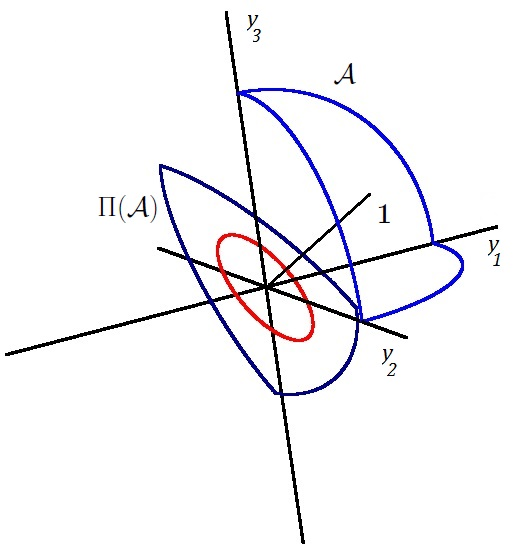
\includegraphics[width=2.5in]{minSS3dSampleSpace.jpg}
\caption{A depiction of $\mathcal{A}$, $\Pi(\mathcal{A})$, and the
  unit circle for the illustrative example where $b_{1}(\mathbf{1},\by)=\min(\by)=0$ and
  $s(\mathbf{1},\by)=\sum (y_i -b_{1}(\mathbf{1},\by))^2 =1$.
$\mathcal{A}$ is the combination of three quarter circles, one
  on each plane defined by $y_i=0$. The projection of this manifold
  onto the deviation space is depicted by the bowed triangular shape
  in the plane defined by $\sum y_i=0$. The circle in this plane
  represents the sample space for the intermediate sample. Also
  depicted is the vector $\mathbf{1}$, the design matrix for the
  location and scale setting.}
\label{fig:sampSpace}
\end{figure}

The set $\mathcal{A}$ typically does not lie in a linear space of dimension $n - p - 1$, and 
so we must account for both the many-to-one nature of the mapping and
a Jacobian when deriving the proposal density.  We handle the first
point by proposing a vector $\bz^*$ 
on an $n - p - 1$ dimensional space which, through a scaling and
shifting, maps to a point 
in $\mathcal{A}$ uniquely.  
The initial proposal is chosen so that the range of the map is the
entirety of $\mathcal{A}$.  The Jacobian does not cancel in
(\ref{MHRatio}), since the scaling depends on the initial proposal. 

Figure~\ref{fig:sampSpace} shows the type of set from which we draw the initial proposal.  Denote the 
column space of the design matrix $X$ by $\mathcal{C}(X)$ and its orthogonal complement by $\mc{C}^\perp(X)$. 
We refer to the latter set as the `deviation space' as it is the space where the traditional least 
squares residuals are contained.  We define the projection of the set $\mathcal{A}$ onto the deviation space as 
\begin{equation}
\label{sampleSpacePerp}
\Pi(\mathcal{A})=\{\bz\in \mathbb{R}^n |\ \exists\ \by\in \mathcal{A}\
s.t.\ \bz=Q \by \}
\end{equation} 
where $Q$ is the projection matrix onto  $\mc{C}^\perp(X)$. Explicitly, $Q=I-H$ with $H=XX^\top$ where we assume without
loss of generality, following condition \ref{fullRank},  that the
columns of $X$ form an orthonormal basis for $\mc{C}(X)$
(i.e., $X^\top X=I$). It will also be helpful at times to write $Q=WW^{\top}$ where the columns of $W$ form an orthonormal basis for $\mc{C}^\perp(X)$. 

The initial proposal is drawn from the surface of the unit sphere in the $n-p$ dimensional $\mc{C}^\perp(X)$.  
In the figure, the column vector $\bf{1}$ spans $\mc{C}(X)$, the triangle with bowed sides is the projection of 
$\mathcal{A}$ onto $\mc{C}^\perp(X)$, and the circle is the set from which the initial proposal is drawn.  

For an initial proposal $\bz^*$ on the surface of the sphere, we move to a point on $\Pi(\mathcal{A})$ through a 
simple scaling of the point $\bz^*$.  This is followed by undoing the projection with a move from 
$\Pi(\mathcal{A})$ to its (unique) preimage on $\mathcal{A}$. Together, these two steps correspond to the
transformation in Theorem~\ref{Transformation}.  The introduction of the initial proposal surface gives us a
1-1 transformation. Properties \ref{regEq}-\ref{scaleEq2Reg} ensure
the mapping described is indeed 1-1. In particular, property
\ref{scaleEq2Reg} ensures the scaling to be unique and \ref{regIn}
implies the scale statistic is unchanged when undoing the
projection. Property \ref{regEq} ensures the uniqueness of undoing the
projection.  
  
The general proposal strategy is summarized as follows
\begin{enumerate}
\item Sample $\bz^*$ from a distribution with known density on the unit sphere in $\mc{C}^\perp(X)$.
\item Implement the transformation in Theorem \ref{Transformation} in two steps
\begin{enumerate}
\item Scale: $\bz=\frac{s(X,\boldsymbol{y}_{obs})}{s(X, \boldsymbol{z}^{*})}\bz^{*}$
\item Shift: $\by=\bz+X\left(\bb(X, \by_{obs})-\bb(X, \bz)\right)$
\end{enumerate}
\end{enumerate}

\subsubsection{Evaluation of the proposal density} 
Calculation of the appropriate Jacobian of the transformation is absolutely vital and also non-trivial. Writing the transformation from the unit sphere in deviation space to $\mathcal{A}$ in 
two steps facilitates calculation 
of the Jacobian in two steps.  

\vskip 0.05 in
\noindent
{\bf From unit sphere to $\Pi(\mathcal{A})$} \\
The first step is constrained to $\mc{C}^\perp(X)$ where the unit sphere is transformed to $\Pi(\mathcal{A})$. We further break this piece in two steps: first, the distribution on the unit sphere is transformed to that along a sphere of radius $r=\|\bz\|={s(X,\boldsymbol{y}_{obs})}/{s(X, \boldsymbol{z}^{*})}$. This contributes $r^{-(n-p-1)}$ to the Jacobian. Second, the new sphere is then deformed to $\Pi(\mathcal{A})$.  This deformation contributes an attenuation to the Jacobian equal to the
ratio of infinitesimal volumes in the
tangent spaces of the sphere and $\Pi(\mathcal{A})$ at $\bz$.  
Restricting ourselves to the $n-p$ dimensional space $\mc{C}^\perp(X)$, this
ratio is the cosine of the angle between the normal 
vectors of the two sets at $\bz$.  The normal to the sphere is $\bz$ and the normal to
$\Pi(\mathcal{A})$ is given in the following lemma.  

\begin{lemma}
\label{gradSTheoremReg}
Assume that conditions \ref{fullRank}-\ref{supReal}, \ref{as}, and \ref{regIn} hold.  
Let $\by\in \mathcal{A}$. Let 
$\nabla s(X,\by)$ denote the
gradient of the scale statistic with respect to the data vector evaluated at
$\by$.  Then $\nabla s(X,\by)\in \mc{C}^\perp(X)$ and is 
normal to $\Pi(\mathcal{A})$ at $\bz=Q\by$  in $\mc{C}^\perp(X)$.
\end{lemma}

The contribution to the  Jacobian of this attenuation is 
\begin{equation}
\label{cosine}
\cos(\gamma)=\frac{\nabla s(X,\by)^\top \bz}{\|\nabla
s(X,\by)\| \|\bz\|},
\end{equation}
where $\gamma$ is the angle between the two normal vectors.
This step is illustrated in Figure~\ref{fig:stretchDeform} for the toy
location-scale example.  

\begin{figure}[!ht]
\centering
\subcaptionbox{}{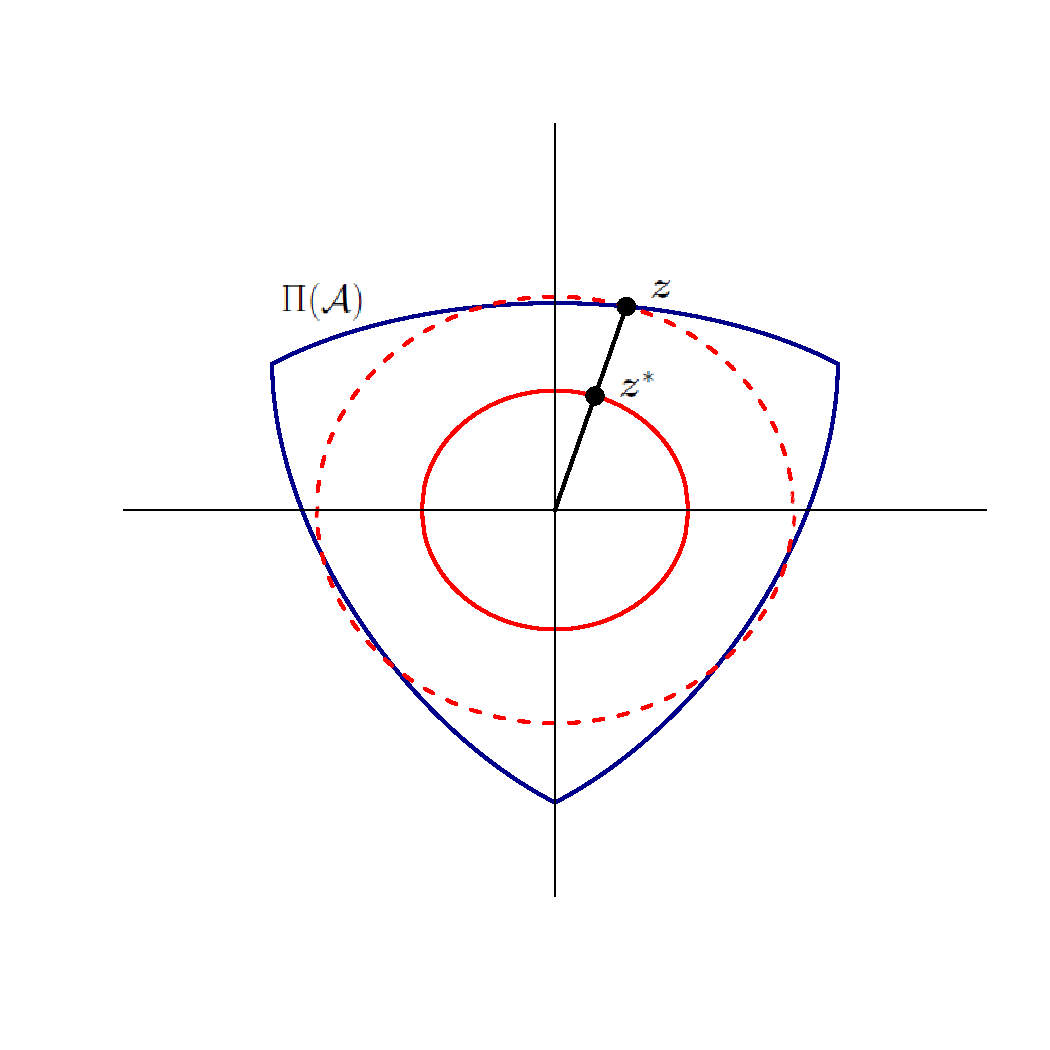
\includegraphics[width=2.5in]{minSSZSpace3.pdf}}\quad
\subcaptionbox{}{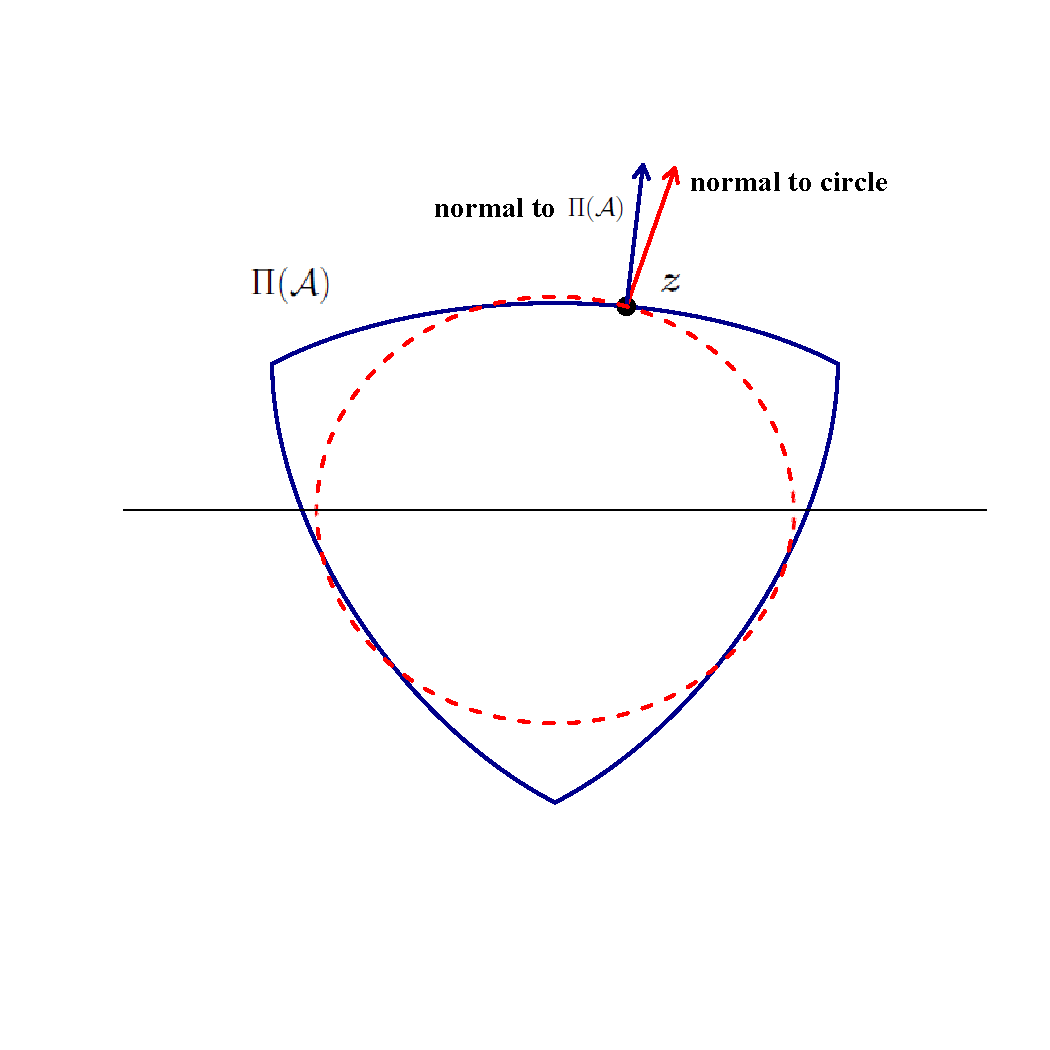
\includegraphics[width=2.5in]{minSSZSpace5.pdf}}
\caption{Panel (a) contains a depiction of the stretch from $\bz^{*}$
  to $\bz$. The adjustment for the stretch transforms the density
  along the unit circle to the density along the circle of radius
  $\|\bz\|$ (dashed circle).  Panel (b) contains a depiction of the
  deformation from the distribution along the circle to the
  distribution along $\Pi(\mathcal{A})$. The adjustment can be seen to
  be the cosine of the angle between the normals to each manifold.}
\label{fig:stretchDeform}
\end{figure}

\vskip 0.05 in
\noindent
{\bf From $\Pi(\mathcal{A})$ to $\mathcal{A}$} \\
The final piece of the Jacobian comes from the transformation from
$\Pi(\mathcal{A})$ to $\mathcal{A}$.  For this we return to the full
$n$ dimensional space.  The second step involves a shift of
$\bz$ to $\by$ along the column space of $X$, but the shift depends on 
$\bz$, and so the density on the set 
$\Pi(\mathcal{A})$ is deformed by the shift. The
contribution of this step to the Jacobian is, from first principles,
the ratio of the infinitesimal volume along $\Pi(\mathcal{A})$ to the
corresponding volume along $\mathcal{A}$. 
The ratio is calculated by considering the volume of the
projection of a unit hypercube in the tangent space of $\mathcal{A}$
at $\by$ onto $\mc{C}^\perp(X)$.
Computational details are
given in the following lemmas and subsequent theorem. Throughout, let
$\mc T_{y}(\mc A)$ and $\mc T_{y}^{\perp}(\mc A)$ denote the tangent
space to $\mc A$ at $\by$ and its orthogonal complement respectively. 

\begin{lemma}
\label{lem:basis}
Assume that conditions \ref{fullRank}-\ref{regEq} and \ref{regIn}-\ref{scaleEq2Reg} hold.  Then the $p+1$ gradient vectors 
$\nabla s(X,\by), \nabla b_1(X,\by),\dots, \nabla b_p(X,\by)$ form a
basis for $\mc T_{y}^\perp(\mc A)$ with probability one.
\end{lemma}

The lemma describes construction of a basis for $\mc T_{y}^\perp(\mc A)$.  This leads to a 
basis for $\mc T_{y}(\mc A)$.  Both of these bases can be orthonormalized.  
Let $B=[b_1,\dots,b_{p+1}]$ and $A=[a_{1},\dots,a_{n-p-1}]$ denote the 
matrices whose columns contain these two orthonormal bases.  
The columns in $A$ define a unit hypercube in $\mc T_{y}(\mc
  A)$ and their projections onto $\mc{C}^\perp(X)$ define a parallelepiped.
We defer construction of $A$ until later.  

\begin{lemma}
\label{lem:fullrank}
Assume that conditions \ref{fullRank}-\ref{regEq} and \ref{regIn}-\ref{scaleEq2Reg} hold.  
Then the $n\times (n-p-1)$ dimensional matrix $P=QA$ is of full column rank.
\end{lemma}

As a consequence of this lemma, 
the parallelepiped spanned by the columns of $P$ is not
degenerate (it is $n-p-1$ dimensional), and its volume
is given by
\begin{equation}
\label{eq:volume}
\text{Vol} (P) := \sqrt{\text{det}(P^\top P)}=\prod_{i=1}^{r} \sigma_i
\end{equation}
where $r=\text{rank} (P)=n-p-1$ and $\sigma_1\geq
\sigma_2\geq\dots\geq\sigma_r>0$ are the singular values of $P$ (e.g.,
\cite{miao1992}). 
Combining Lemmas \ref{lem:basis} and \ref{lem:fullrank} above leaves us with the following result concerning the calculation of the desired Jacobian.  
\begin{theorem}
\label{Jacobian}
Assume that conditions \ref{fullRank}-\ref{regEq} and \ref{regIn}-\ref{scaleEq2Reg} hold.  Then the
Jacobian of the transformation from the distribution along 
$\Pi(\mc A)$ to that along $\mc A $ is equal to the volume given in \eqref{eq:volume}.
\end{theorem}

\vskip 0.05 in
\noindent
{\bf The proposal density} \\
Putting all the pieces of the Jacobian together we have the following result. Any dependence on other variables, including current states in the Markov chain, is made implicit. 
\begin{theorem} 
Assume that conditions \ref{fullRank}-\ref{scaleEq2Reg} hold.  Let $\bz^{*}$ be sampled on the unit sphere in $\mc {C}^\perp (X)$ with density $p(\bz^{*})$.  Using the transformation of $\bz^*$ to $\by\in \mc A$ described in Theorem \ref{Transformation}, the density of $\by$ is
\begin{equation}
\label{dens:ystst}
p(\by)=p(\bz^*) r^{-(n-p-1)} \cos(\gamma)\text{Vol} (P)
\end{equation}
where $r={s(X,\boldsymbol{y}_{obs})}/{s(X,  \boldsymbol{z}^{*})}$,
and $\cos(\gamma)$ and $\text{Vol} (P)$ are as in equations \eqref{cosine} and \eqref{eq:volume} respectively. 
\end{theorem} 

In practice, computing $A$ is computationally intensive as it involves orthogonalization of $n$ vectors in $n$-dimensional space. 
To find a matrix $A$, supplement $B$ with a set of $n$ linearly independent columns on the right, and apply Gram-Schmidt 
orthonormalization to the matrix.  This algorithm is slow when $n$ is large, as it is $\mc O(n^3)$ and $A$ must be found at each
iterate of the algorithm when a complete data set is drawn.  
Fortunately, we can make use of results related to \textit{principal angles} found in \cite{miao1992} to compute the volume in \eqref{eq:volume} using $B$ and an orthonormal basis for $\mc C (X)$ (The definition of principal angles can be found in the cited text). Recall, $B$ is constructed by orthogonalization of a basis for $\mc T_{y}^\perp(\mc A)$. Since this space is of dimension $p+1$, applying Gram-Schmidt to find the orthonormal basis is much faster, the algorithm is $\mc O(np^2)$, and there is a 
considerable reduction in computational burden when $n \gg p$. 
Further, the singular values of $P$ are also the singular values of
$W^\top A$, which can be easily obtained through $B$.
The following corollary formally states how computation of $A$ can be circumvented. 
\begin{corollary}
\label{theorem:sings}
Let $U$ be a matrix whose columns
form an orthonormal basis for $\mc C (X)$. Then the non-unit singular
values of $U^\top B$ are the same as the non-unit singular values of $W^\top A$.  
\end{corollary}

%%%%%%%%%%%%%%%%%%%%%%%%%%%%%%%%%%%%%%%%%%%%%%%%%%%%%%%%%%%%
%
% Applications
%
%%%%%%%%%%%%%%%%%%%%%%%%%%%%%%%%%%%%%%%%%%%%%%%%%%%%%%%%%%%%
\section{Applications}
\label{Applications}
We illustrate the methods developed in Sections~\ref{restrictedlikelihood} and \ref{BayesLinMod} with a pair of regression models for 
data from Nationwide Insurance Company, which concern prediction of
the performance of insurance agencies.
The data contain outliers and are subject to model misspecification.  
In particular, a group of the data do not follow the same generative process as the data of interest.  It would be 
extremely challenging to model some features of the data.  
In our analysis, we follow the standard practice when demonstrating the benefits of robust 
methods.  We work with a naive model for the data which ignores certain features of the problem.  We
do this both to create a situation where all can agree that the model for the complete data $\by$ is imperfect
and to preserve the confidentiality of selected aspects of modelling done by Nationwide.  
We wish to provide inference for the `good' portion of the data.  The two models we fit either treat the analysis
as a single regression or as a collection of related regressions.  Details of the models, prior distributions, 
and conditioning statistics are given in the next two subsections.  

%%%%%%%%%%%%%%%%%%%%%%%
%NW data
%%%%%%%%%%%%%%%%%%%%%%%

\subsection{Nationwide Data}
The Nationwide Insurance Company sells many of its insurance policies through agencies which provide direct service to policy holders.  
The contractual agreements between Nationwide and these agencies vary.  Of major interest to Nationwide is the prediction of future performance of agencies where, for our purposes,  performance is measured by the total number of households an agency services (`household count'). A serviced household is one in which at least one person living at that residence has at least one policy written through the agency. We used data from previous years to build a model to forecast future household count. In particular, we use agency characteristics, as measured during a single month in $2010$, to predict household counts in the corresponding month in $2012$. The characteristics used are household count and two measurements of agency size/experience. The two measurements of agency size/experience are, roughly, the number of employed persons at the agency and the length of time the agency has been affiliated with Nationwide. The household counts (response and predictor) have been square rooted to stabilize variance. The data are 
proprietary, and to mask them all variables have been individually centered and scaled and identifiers (agency/agent names and state
labels) have been removed. 
All subsequent analysis is done on this scale.  As an exploratory view, a plot of the square root of count in 2012, against that in 2010 
is shown in Figure \ref{fig:ctVct}.  The different colors represent the varying contractual agreements as they stood in 2010. `Type 1' agencies are of special interest.  Among the open agencies, a strong linear correlation exists.  The specific linear relationship
depends on agency type. The data are characterized by a large number of agencies which were open in 2010 but closed sometime before 2012, as represented by the horizontal band at $0$. We use these data as a test bed for our techniques, fitting models that do not account for agency closures or contract type.  Our expectation is that the restricted likelihood will facilitate prediction for the good part of the data.  

\begin{figure}[t]
\centering
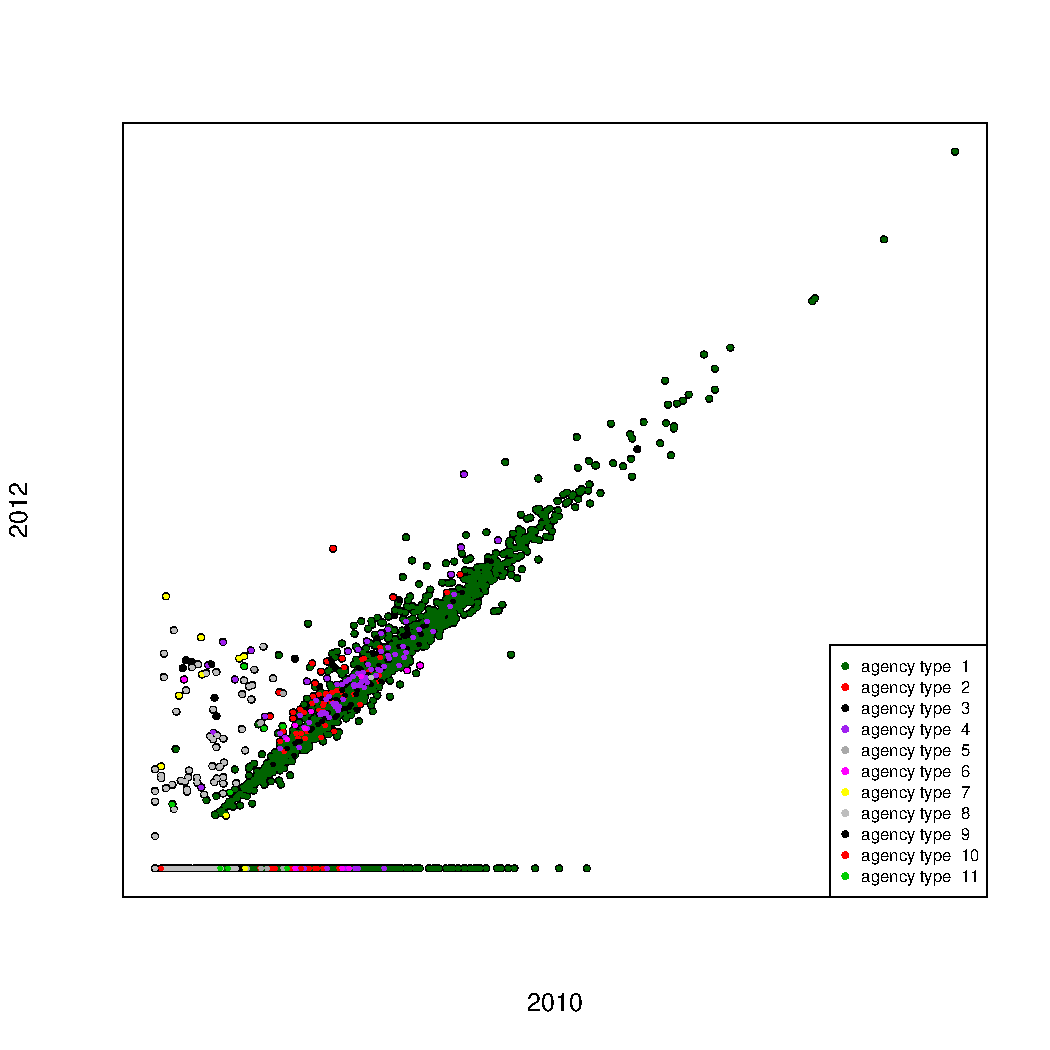
\includegraphics[width=2.8in]{countvcount.pdf}
\caption{The square root of count in 2012 versus that in 2010 (after centering and scaling). The colors represent the varying contractual agreements as they stood in 2010.  Agencies that closed during the 2010-2012 period are represented by the zero counts for 2012.}
\label{fig:ctVct}
\end{figure}

\subsection{Regression model}
The first analysis that we consider is based on a single regression.  We use 
the following standard normal theory regression model 
\begin{equation}
\label{eq:regModel}
\bbeta\sim N_p(\mu_0, \Sigma_0);\ \ \sigma^2\sim IG(a_0,b_0);\ \  
y_{i}=\bx_{i}^\top\bbeta+\epsilon_{i},\ \ \epsilon_{i}\iid N(0, \sigma^2),\ i=1,\dots, n, 
\end{equation}
where $\bbeta$ is a four dimensional vector ($p=4$) of regression coefficients for the intercept, square root of count in 2010, and the two size/experience measures, and $y_{i}$ is the square rooted household count in 2012 for the $i^{th}$ agency with covariate vector $\bx_{i}$.  Although the mean of covariates and response have been removed, we include the intercept as fitting is done on a holdout set to evaluate predictive performance.  
The hyper-parameters $a_0, b_0, \bmu_0$ and $\Sigma_0$ are all fixed and set from a 
robust regression fit to the data from the time period two years
before. $\mu_0$ is set to the estimate of the regression
coefficients. $\Sigma_0$ is set to $n\cdot \mbox{var}(\bb)$
where $n$ is taken as the sample size of the prior data set, corresponding to  a unit information prior for $\bbeta$. The hyperparameters for $\sigma^2$ are set so that the prior mean is $s^2$, the estimated variance from the robust regression, and the spread of the prior covers the range of plausible values with high probability. All values are then transformed appropriatly to match the current scale of the data. In the end we take $\mu_0=(0.18,  0.81,0.01,-0.02)^\top$ and set the mean of $\sigma^2$ to $0.014$ and standard deviation to  $0.033$. 

We compare four Bayesian models: the standard Bayesian normal theory model, two restricted likelihood models, both with simultaneous M-estimators as the restriction, and a heavy tailed model. The heavy-tailed model replaces the normal sampling density in \eqref{eq:regModel} with a $t$-distribution with $\nu = 3$ degrees of freedom. The restricted likelihood methods use 
standard $\rho$ functions, colloquially known as Huber's $\rho$ and Tukey's $\rho$.  We have used the default tunning parameter settings for the {\tt rlm} function in the R package {\tt MASS} \citep{venables2002}.  Both use Huber's scale estimator as in the {\tt rlm} implementation.  We also fit the corresponding classical robust regressions and a least squares regression.  

\subsubsection{Method of model comparison}
We wish to examine the performance of the models in a fashion that preserves the essential features of the 
problem.  Since we are concerned with outliers and model 
misspecification, we understand that our models are imperfect and so prefer to use an out-of-sample measure of fit.  
This leads us to cross-validation.  We repeatedly split the data into training
and validation sets.  We fit the model to the training data and assess its performance on the validation data.  

The presence of numerous outliers in the data implies that both training and validation data will contain 
outliers.  For this reason, the evaluation must be robust to a certain fraction of bad data.  
The two main strategies are to robustify the evaluation function \citep[e.g.,][]{ronchetti1997} or 
to retain the desired evaluation function and trim cases \citep{jung2014}.  Here,
we pursue the trimming approach with log predictive density for the Bayesian models and log plug-in 
maximum likelihood for the classical fits. 

The trimmed evaluation proceeds as follows in our context.  The evaluation function for case $i$ in the hold-out data
is the log predictive density, say
$\log(f(y_i))$, with the conditioning on the training data suppressed.  The trimming 
fraction is set at $0 \leq \alpha < 1$. To score a method,
we first identify a base method.  Under the base method, $\log(f(y_i))$ is computed for each case in the 
validation sample, say $i = 1, \ldots, M$.  The $[\alpha M]$ observations with the smallest values of $\log(f(y_i))$ are 
removed from the validation sample.  All of the methods are then scored on the
remaining $M - [\alpha M]$ observations in the validation sample with the mean trimmed log marginal pseudo likelihood, 
$TLM = (M - [\alpha M])^{-1} \sum \log(f(y_i))$.  
The sum runs over the remaining observations.  This process is advantageous to the base method.  A method
that performs poorly when it is the base method is discredited.  For a complete evaluation, we allow each method
to appear as the base method.  For brevity, we present only a selection of results in our subsequent analyses.  

\subsubsection{Comparison of predictive performance}
Model performance is assessed
using the mean and standard deviation of the TLM 
across $100$ different replicates. First, we include all observations
in each validation sample to calculate TLM for each split. We then
repeat the evaluation using only certain subsets of the validation
sample that are of special interest. Subsets include open agencies,
open `Type 1' agencies, and `Type 1' agencies. For brevity, we include
results for the `Type 1' agencies only. As noted, assessing model
predictions on this set of agencies is of special interest to the
company.  A range of training sample sizes were used and we include
results from $n=25,100,1000,$ and $2000$ out of a total of $3180$ agencies. The trimming fraction, $\alpha$, ranges from $0$ to $0.3$. A classical robust regression to the prior data assigns zero weight to around $16\%$ of observations; in essence removing these from the analysis. This informed the range of trimming fractions chosen.  
In practice, we would set $\alpha$ slightly larger than $0.16$.  

\begin{figure}[t]
\centering
\subcaptionbox{}{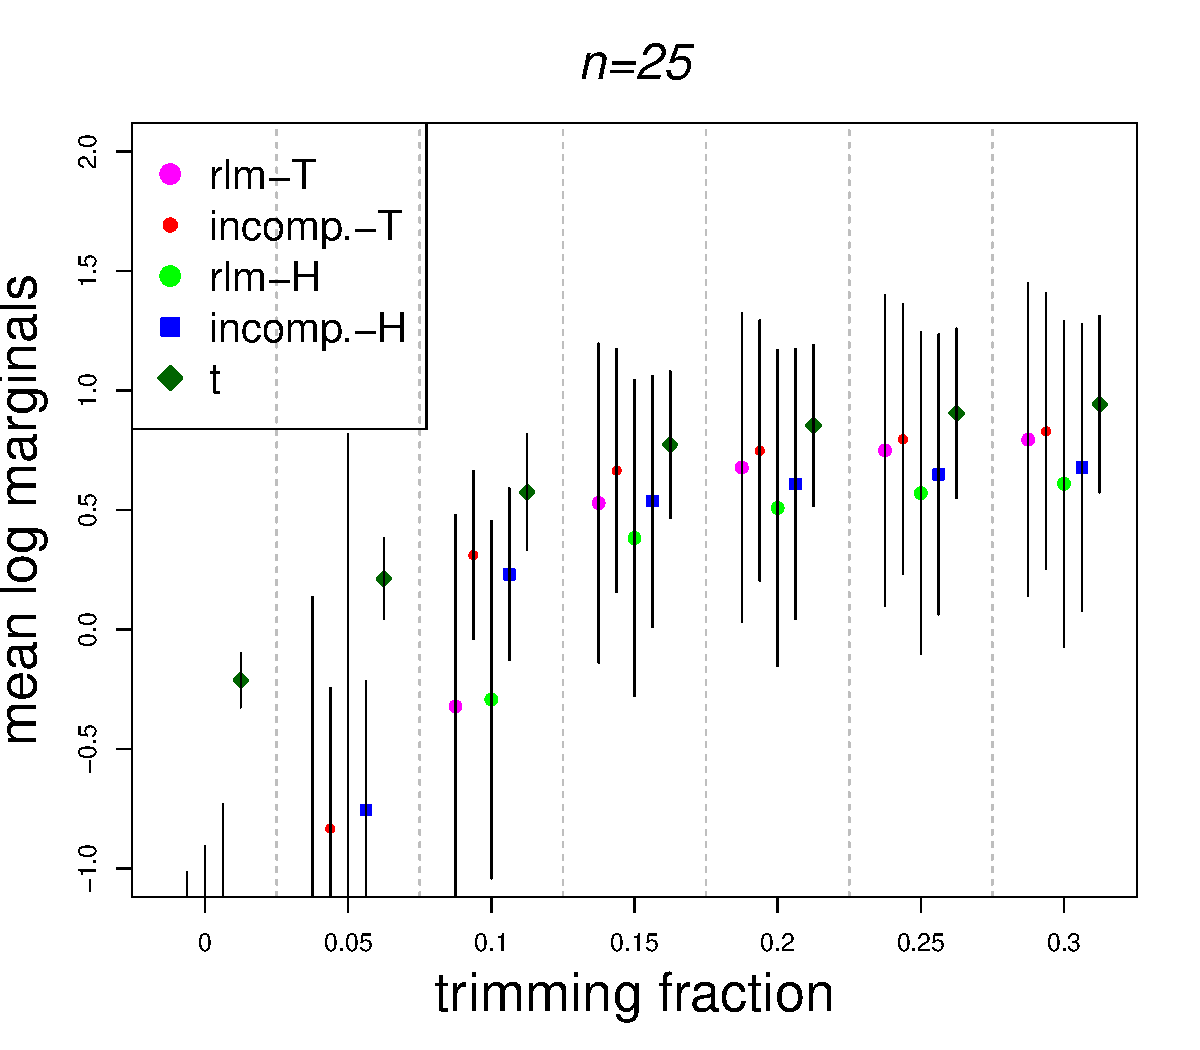
\includegraphics[width=.31\textwidth,page=1]{logMargType1AgenciesBaseModelt}}\quad
\subcaptionbox{}{\includegraphics[width=.31\textwidth,page=2]{logMargType1AgenciesBaseModelt}}\quad
\subcaptionbox{}{\includegraphics[width=.31\textwidth,page=3]{logMargType1AgenciesBaseModelt}}
\caption{Model evaluation for `Type 1' agencies for training sample
  sizes of $n=25,100$, and $1000$. The $t$-model is used as the base
  method to compute TLM. Plotted are the mean TLM for each model
  against the trimming fraction across the $100$ cross-validation
  samples. Error bars correspond to one standard deviation of TLM
  above and below the mean. Models are labeled with the following
  abbreviations: `rlm' corresponds to a classical robust fit, `rest.'
  corresponds to our restricted method, and `t' corresponds to the
  heavy-tailed $t$-distribution model. The letters `T' and `H'
  appearing after `rlm' and `rest.' correspond to the use of  Tukey's
  and Huber's $\rho$ respectively. 
}
\label{fig:Type1Marg}
\end{figure}


Model evaluation for `Type 1' agencies is shown in Figure
\ref{fig:Type1Marg} for training sample sizes $n=25, 100,$ and $1000$.
The normal theory models perform poorly due to the numerous outliers
and are left out. Appearing in the figures are the mean TLM across
each validation set for each model and each trimming fraction, $\alpha$ (along the $x$-axis). The error bars depicted are one standard deviation of the TLM above and below the mean. The models pictured are: classical robust regression with Tukey's $\rho$ (rlm-T), restricted likelihood based on the `Tukey estimate' (rest.-T), classical robust regression with Huber's $\rho$ function (rlm-H), restricted likelihood based on the `Huber estimate' (rest.-H), and the thick tailed t-model (t). The range of the vertical axis is chosen to enhance important features and as a result, some evaluation measures extend below this range. In particular, the restricted methods perform poorly if no  trimming is done; reflecting that these methods are not intended to fit well to outliers. Recall that we expect about 15-16\% outliers in the validation sets, thus trimming fractions slightly larger than this amount are needed in order to assess fits to the `good' data. For $n=25$, the thick tailed model  prevails across trimming fractions, although less so for $\alpha\geq 0.15$. For sample sizes as low as $n=100$, the restricted methods outperform the thick tailed model with the Tukey version performing the best.   
The stronger performance of restricted likelihood based on Tukey's method and the t model is to be expected, as many of the 
residuals are so extreme that trimming is better than winsorizing (as Huber's method effectively does).  
As expected, with enough data,  the Bayesian methods and their classical counterparts perform similarly, although there
is a persistent slight edge in favor of the restricted likelihood methods.  We attribute this advantage to the weakly informative
prior distribution which pulls the estimates slightly toward better values.  The similarity occurs as early as $n=100$. 

 
\subsection{Hierarchical regression model}
Nationwide agencies span many states and insurance regulations and the competitive environment varies between states. A natural extension to the previous analysis is a hierarchical regression model, grouping agencies within each state to reflect similar business environments. Using the same study design with the same training and validation splits, we re-analyze the data using the following hierarchical regression model:
\begin{align}
\label{eq:hierModel}
&\bbeta\sim N_p(\mu_0, a\Sigma_0);\ \ 
\bbeta_j\iid N_p(\bbeta, b\Sigma_0);\nonumber \ \  
\sigma_j^2\sim IG(a_0,b_0);  & \\ 
& \by_{ij}=\bx_{ij}^\top\bbeta_j+\epsilon_{ij},\ \ \epsilon_{ij}\iid N(0, \sigma_j^2),\ i=1,\dots, n_j,\ j=1,\dots, J & \nonumber
\end{align}
where $y_{ij}$  represents the $i^{th}$ observation in the $j^{th}$
state, $n_j$ is the total number of agencies in each state, and $J$ is
the number of states. $\bx_{ij}$ is a four dimensional vector
comprised of the same covariates as above. $\bbeta_j$ represents the
individual regression coefficient vector for state $j$.  We match this
model to the non-hierarchical model in several ways. First, $\mu_0$,
$\Sigma_0$, $a_0$, and $b_0$ are fixed as before. We constrain $a+b=1$
in an attempt to partition the total variance between the individual
$\bbeta_j$'s and the overall $\bbeta$. We take $b\sim
\text{beta}(v_1,v_2)$. Using the previous data set, we assess the
variation between individual estimates of the $\beta_j$ to set $v_1$
and $v_2$ to allow for a reasonable amount of shrinkage. To allow for
dependence across the $\sigma_j^2$ we first take
$(z_1,\dots,z_J)\sim N_J(\mathbf{0}, \Sigma_\rho)$ with
$\Sigma_\rho=(1-\rho)I+\rho J$. Then we set
$\sigma^2_j=H^{-1}(\Phi(z_j))$ where $H$ is the cdf of an
$IG(a_0,b_0)$ resulting in the specified marginal distribution, while
introducing correlation via $\rho$. We assume $\rho\sim
\text{beta}(a_\rho,b_\rho)$ with mean $\mu_\rho$ and precision
$\psi_\rho=a_\rho+b_\rho$. The parameters $\mu_\rho$ and
$\psi_{\rho}$  are given beta and gamma distributions respectively, both with fixed hyperparameters. To choose these fixed values we again consider fits to individual states from the previous dataset. Plugging the estimates of $z_j$ into the multivariate normal, the mean of $\mu_\rho$ is set to the MLE of $\rho$ and the variance is set to the observed inverse Fisher information matrix, inflated by a factor of $2$ to weaken the prior for this parameter.  We use the same MLE and inflated information matrix to set the mean for $\psi_{\rho}$. Its variance is chosen to cover a range of plausible values. A range of other values for the fixed hyper-parameters was also studied.  The differences in results were negligible. 

Using the same techniques as in the previous section, 
we fit the normal theory hierarchical model above, a thick tailed $t$ version with $\nu = 3$ d.f., and two restricted likelihood versions (Huber's and Tukey's) of the model.  For the restricted likelihood methods, we condition on robust regression estimates fit separately within each state. Both use Huber's scale estimator. We also fit classical robust regression counterparts and a least squares regression separately within each state.  

We digress briefly to note that no additional computational strategies outside of those discussed in Section~\ref{highDim} are needed to fit the restricted hierarchical models described here. Since we condition on statistics which are computed within each state, the model's conditional independence between the states allows the data augmentation described earlier to be performed independently within each state.  Updates of hyperparameters follow conventional MCMC procedures.  We note that different types of statistics could be chosen for each state, if desired, allowing for a large amount of flexibility.  

Selected results for the hierarchical fits appear in Figure \ref{fig:hierType1Marg}. Hierarchical models naturally require more data and so we consider only training sizes of $n=1000$ and $2000$. Trimming fractions between $0.15$ and $0.3$ are displayed as patterns for smaller trimming fractions are similar to those from the non-hierarchical fits. That is, without sufficient trimming, the restricted likelihood fits' evaluation measure is poor. Again, the normal theory fits, both Bayesian and classical, perform poorly and are left out of the figures.  We see that Tukey's version of restricted fits performs best in each case (assuming sufficient trimming). Huber's version also tops the thick tailed model for $n=2000$.  The Bayesian restricted fits considerably outperform their respective individual classical robust fits for training size of $n=1000$. This observation remains, though marginally so, for $n=2000$. The advantage of the hierarchical models seen here is due to the pooling of information across states, resulting in better predictive performance as compared to both the thick tailed competitor as well the respective classical fits.

\begin{figure}[t]
\subcaptionbox{}{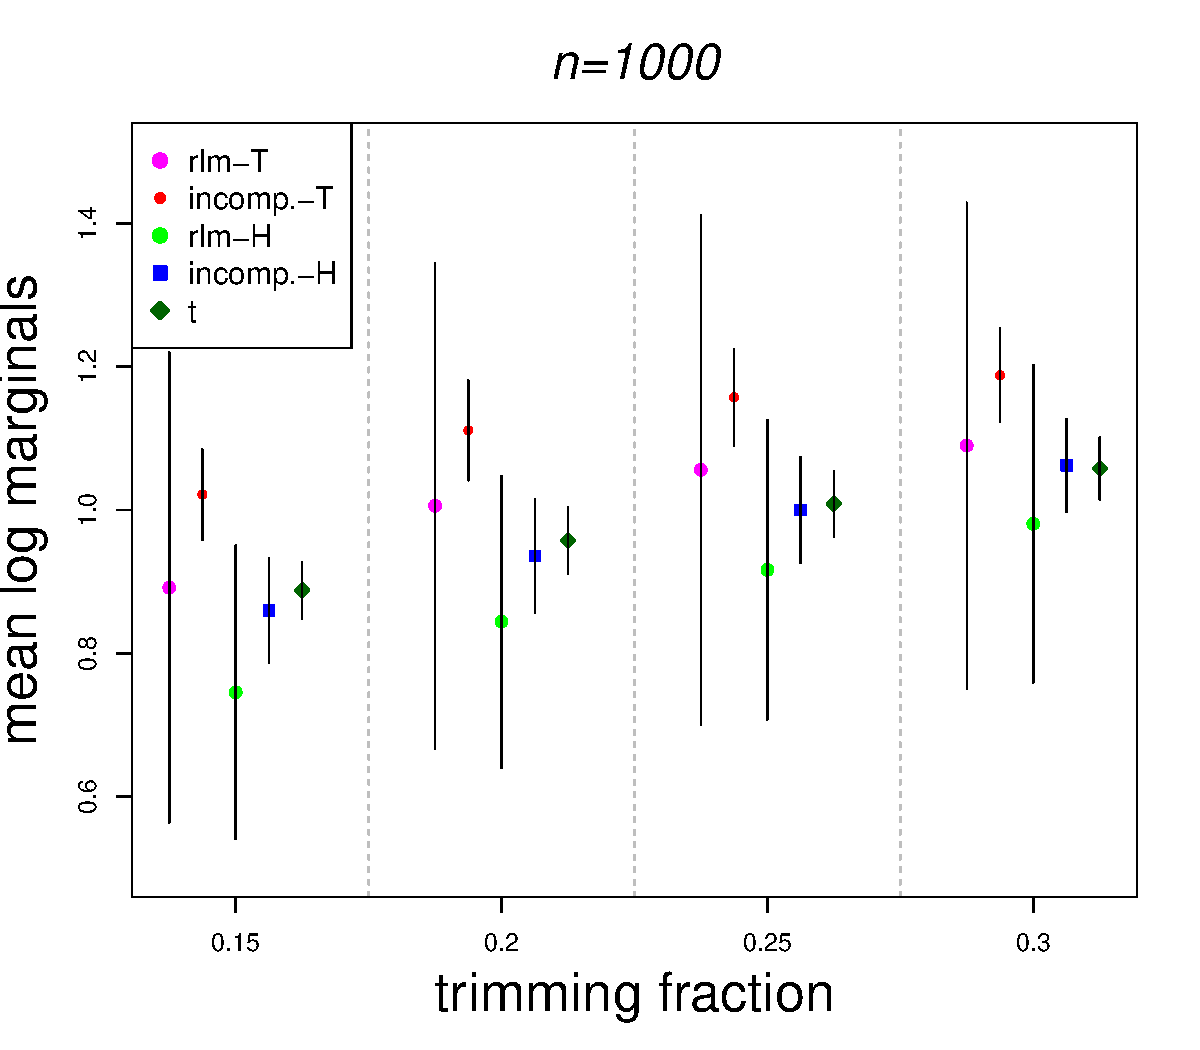
\includegraphics[width=2.75in,page=1]{hierlogMargType1AgenciesBaseModelt}}\quad
\subcaptionbox{}{\includegraphics[width=2.75in,page=2]{hierlogMargType1AgenciesBaseModelt}}
\caption{Model evaluation for `Type 1' agencies under the hierarchical model for $n=1000$ and $2000$. The $t$-model is used as the base method to compute TLM. Plotted are the mean TLM for each model against the trimming fraction across the $100$ cross-validation samples. Error bars correspond to one standard deviation of TLM above and below the mean. Models are labeled using the same notation as the previous figure. Only the relevant trimming fractions ($\alpha\geq .15$) are pictured.  
}
\label{fig:hierType1Marg}
\end{figure}


\subsection{Comparison of hierarchical and non-hierarchical fits}

The performance of the methods for the hierarchical and non-hierarchical models can be contrasted through our cross validations studies.  We focus on Tukey's and Huber's conditioning statistic and concentrate our evaluation on the `Type 1' agencies. Table~\ref{tab:tlmTable} displays the mean TLM for each model and range of trimming fractions.  Our summary below focuses exclusively on realistic trimming fractions, $\alpha \geq 0.15$, and Tukey's conditioning statistic.  

We first note that for the non-hierarchical model, there is little difference between mean TLM for $n=1000$ and $n=2000$, with 
the numbers differing only in the third decimal place.  This is due to the posterior predictive distributions having stabilized.  The
mean TLMs for the hierarchical model show a greater change with increases of about $0.05$ to $0.07$ as the training sample size changes
from $1000$ to $2000$.  For calibration, the mean TLM for a normal with mean $0.5$ and variance $1$ is approximately this size
when trimming is done under a standard normal base model.  Thus, the increase in mean TLM is substantial.  
We attribute the change for the hierarchical model to the 
improvement in fits, particularly for states with fewer agencies.  

Direct comparison of the hierarchical and non-hierarchical models shows that, for $n=1000$, the non-hierarchical model has uniformly 
(for $\alpha$ of interest) better mean TLM.  The differences are substantial, and the summaries primarily reflect greater stability of fits on a state-by-state basis under the non-hierarchical model.  To a lesser extent, they reflect variation in the evaluation criterion which stems from modest validation sample size, particularly with larger trimming fractions.  The trimmed cases are not proportionally distributed across states.  The pattern changes for $n=2000$, with the hierarchical model showing larger mean TLMs for trimming fractions $0.15$ and $0.20$.  The improvement reflects the ability of the hierarchical model to capture differences in regressions across the states which is realized when the training sample size is large enough.  We attribute the better performance of the non-hierarchical model for the largest trimming fractions to variation in the evaluation.  

\begin{table}[!tbp]
{\small
\begin{center}
\begin{tabular}{lllll}
\hline\hline
& \multicolumn{4}{c}{Trimming fraction ($\alpha$)}\\
\multicolumn{1}{l}{}&\multicolumn{1}{c}{$0.15$}&\multicolumn{1}{c}{$0.2$}&\multicolumn{1}{c}{$0.25$}&\multicolumn{1}{c}{$0.3$}\tabularnewline
\hline
{\mdseries Tukey ($n=1000$)}&&&&\tabularnewline
~~Non-Hier.&1.072 (0.014)&1.179 (0.022)&1.226 (0.029)&1.255 (0.033)\tabularnewline
~~Hier.&1.021 (0.063)&1.110 (0.070)&1.157 (0.067)&1.187 (0.065)\tabularnewline
\hline
{\mdseries Tukey ($n=2000$) }&&&&\tabularnewline
~~Non-Hier.&1.068 (0.029)&1.178 (0.007)&1.225 (0.011)&1.254 (0.014)\tabularnewline
~~Hier.&1.094 (0.041)&1.189 (0.036)&1.221 (0.033)&1.242 (0.028)\tabularnewline
\hline
{\mdseries Huber  ($n=1000$)}&&&&\tabularnewline
~~Non-Hier.&1.020 (0.020)&1.114 (0.035)&1.157 (0.041)&1.184 (0.045)\tabularnewline
~~Hier.&0.861 (0.073)&0.937 (0.079)&1.001 (0.074)&1.063 (0.064)\tabularnewline
\hline
{\mdseries Huber ($n=2000$)}&&&&\tabularnewline
~~Non-Hier.&1.015 (0.021)&1.112 (0.014)&1.154 (0.019)&1.181 (0.023)\tabularnewline
~~Hier.&0.930 (0.041)&1.014 (0.043)&1.080 (0.035)&1.148 (0.027)\tabularnewline
\hline
\end{tabular}
\end{center}
\caption{Mean (standard deviation) of TLM for `Type 1' agencies for the restricted non-hierarchical and hierarchical models for $n=1000$ and $2000$.} \label{tab:tlmTable}
}
\end{table}


\section{Discussion}
\label{Conclusions}

In this work, we have presented an approach which begins to reconcile
Bayesian methods with the practice of data analysis.  Many routine
choices in an analysis react to the gap between reality and the
statistical model, where a bit of set-up work improves inferential
performance.  Often, these choices can be recast in the framework of
restricted likelihood, lending them more formality and facilitating
development of theoretical results.  But a much greater benefit of our
framework is that it leads us to blend classical estimation with
Bayesian methods.  Here, we use the likelihood from robust regression
estimators to move from prior distribution to posterior distribution.
Conditioning on the estimator, the update follows Bayes' Theorem
exactly.   Computation is driven by MCMC methods, requiring only a modest supplement to existing algorithms.  In another context, we might condition on the results of a set of estimating equations, designed to enforce lexical preferences for those features of the analysis considered most important, yet still producing inferences for secondary aspects of the problem.  In other settings, we envision conditioning on a mix of estimators and some of the observed data.  

The framework we propose allows us to retain many benefits of Bayesian methods:  it requires a full and complete model for the data; it lets us combine various sources of information both through the use of a prior distribution and through creation of a hierarchical model; it guarantees admissibility of our decision rules among the class based on the summary statistic $T(\by)$; and it naturally leads us to focus on predictive inference.   

This same framework retains many of the benefits of classical estimation.  Great ingenuity has been used to create a wide variety of estimators in this tradition, many of which are designed to handle specific flaws in the model.  The estimators are typically accompanied by asymptotic results on consistency and distribution.  Many of these results carry over to our blend of classical and Bayesian methods, although regularity conditions differ.  We expect our procedures to have strong large sample performance, especially in settings where
pooling of information is of value.  

This framework opens a number of questions, including a need to revisit such issues as model selection, model averaging for predictive performance, and the role of diagnostics.  Perhaps the biggest question is which summary statistic to choose.  For this, we recommend a choice based on the analyst's understanding of the problem, model, reality, deficiencies in the model,  inferences to be made, and the relative importance of various inferences. 


\section{Appendix}
\label{sec:appendix}

\noindent
Proof of Theorem~\ref{Transformation}.  
\begin{proof} 
\begin{eqnarray}
 s(X,\by) & = & \frac{s(X,\by_{obs})}{s(X,\by^*)} s(X, \by^*)= s(X,\by_{obs}) , \qquad \mbox{and} \\
 \bb(X,\by) & = & \bb\left(X,\frac{s(X,\by_{obs})}{s(X,\by^*)}\by^* + X\left(\bb(X,\by_{obs}) - \bb(X,\frac{s(X,\by_{obs})}{s(X,\by^*)}\by^*)\right)\right) \\
 & = & \bb(X,\frac{s(X,\by_{obs})}{s(X,\by^*)}\by^*) + \bb(X,\by_{obs}) - \bb(X,\frac{s(X,\by_{obs})}{s(X,\by^*)}\by^*) \\ &=& \bb(X,\by_{obs})
\end{eqnarray}
\end{proof}

\noindent
Proof of Lemma~\ref{gradSTheoremReg}.
\begin{proof}
We first show that $\nabla s(X,\by)\in \mc{C}^\perp(X)$. Recall that
$H=I-Q$. By the regression invariance property \ref{regIn} of $s$, we have
\label{perpGradReg}
\begin{equation}
\label{eq:lem3.2}
\begin{aligned}
s(X,\by)=s(X, Q\by+H\by)=s(X, Q\by).
\end{aligned}
\end{equation}
Thus, by the chain rule $\nabla s(X,\by)=Q\nabla s(X,Q\by)=Q\nabla s(X, \bz)$. Hence $X^\top \nabla s(X,\by)=0$ as desired.
From equation~\eqref{eq:lem3.2}, all vectors $\bz'\in \Pi(\mathcal{A})$ satisfy $s(X,\bz')=
s(X,\by)=s(X,\by_{obs})$, and so all directional derivatives of $s$ along each tangent $\bv$ to
  $\Pi(\mathcal{A})$ in $\mc C^\perp(X)$ at $\bz$ are equal to 0 (i.e., $\nabla s(X,\bz) \cdot \bv=0$).  Thus $\nabla s(X,\bz)$ is orthogonal to  $\Pi(\mathcal{A})$ at $\bz$.  
Since $\Pi(\mathcal{A})$ has dimension $n-p-1$, $\nabla s(X,\bz)$ gives the unique (up to scaling and reversing direction) normal in the $n-p$ dimensional $\mc C^\perp(X)$.  
\end{proof}

\noindent
Proof of Lemma~\ref{lem:basis}

\begin{proof}
Without loss of generality, assume the columns of $X$ form an
orthonormal basis for $\mc C (X)$ and likewise the columns of $W$ form
and orthonormal basis for $\mc C^\perp(X)$. With earlier notation,
$H=XX^{\top}$ and $Q=WW^{\top}$. The set $\mc A$ is defined by the
$p+1$ equations  $s(X,\by)=s(X,\by_{obs})$, 
$b_1(X,\by)=b_1(X,\by_{obs}),\dots,  b_p(X,\by)=b_p(X,\by_{obs})$. Consequently, the gradients are orthogonal to $\mc A$. Let  $\nabla\bb(X,\by)$ denote the $n\times p$ matrix with columns $\nabla b_1(X,\by),\dots, \nabla b_p(X,\by)$. We seek to show the $n \times (p+1)$ matrix $[\nabla\boldsymbol\bb(X,\by),\nabla s(X,\by)]$ has rank $p+1$. Using property \ref{regEq}, we have that 
\[
\bb(X, \by)=\bb(X,Q\by+H\by)=\bb(X, Q\by)+X^\top \by
\] 
Then $\nabla \bb(X,\by)=Q\nabla\boldsymbol\bb(X, Q\by)+ X$ and 
\begin{eqnarray}
\label{BigMatrix}
[XX^\top, WW^\top]^\top[\nabla\boldsymbol\bb(X,\by),\nabla s(X,\by)]=
 \left( \begin{array}{cc}
X & \mathbf{0} \\
WW^\top\nabla b(X,\by)  &\nabla s(X,\by)  \\ \end{array} \right)
\end{eqnarray}
The last column comes from Lemma \ref{gradSTheoremReg}. The matrix $[XX^\top, WW^\top]^\top$ is of full
column rank (rank $n$), and so the rank of $[\nabla\boldsymbol\bb(X,\by),\nabla s(X,\by)]$ is the same as the rank
of the matrix on the right hand side of (\ref{BigMatrix}).  This last
matrix has rank $p+1$ since $\nabla s(X,\by) \ne \bzero$ by \ref{scaleEq2Reg}, and so does 
$[\nabla b(X,\by),\nabla s(X,\by)]$.
\end{proof}

\noindent
Proof of Lemma~\ref{lem:fullrank}

\begin{proof}
$P$ is the projection of the columns of $A$ onto $\mc
C^{\perp}(X)$. For this to result in a loss of rank, a subspace of
$\mc T_{y}(\mc A)$ must belong to $\mc C(X)$.  Following property
\ref{regEq}, for an arbitrary vector $X \bv \in \mc C(X)$, $\bb(X,\by
+ X \bv) = \bb(X,\by) + \bv$.  From the property, we can show that the directional derivative
  of $\bb$ along $X \bv$ with $\bv \ne \bzero$ is $\bv$, which is a
  nonzero vector. Hence $X\bv \notin \mc T_{y}(\mc A)$.  
\end{proof}

\noindent
Proof of Corollary~\ref{theorem:sings}

\begin{proof}
The corollary relies on a lemma and theorem from \cite{miao1992} which we restate 
slightly for brevity of presentation.  The principal angles between subspaces pluck off a
set of angles between subspaces, from smallest to largest.  The number of such angles 
is the minimum of the dimensions of the two subspaces.  Miao and Ben-Israel's first result
(their Lemma 1) connects these principal angles to a set of singular values, and hence to 
volumes.   
\begin{lemma}{(Miao, Ben-Israel)}
\label{MBI:lemma}
Let the columns of $Q_L\in \mathbb{R}^{n\times l}$ and $Q_M\in
\mathbb{R}^{n\times m}$ form orthonormal bases for linear subspaces
$L$ and $M$ respectively, with $l \leq m$. Let $\sigma_1\geq\cdots\geq
\sigma_l\geq0$ be the singular values of $Q_M^\top Q_L$. Then $\cos
\theta_i=\sigma_i, i=1,\dots,l$ where $0\leq\theta_1\leq\theta_2\leq
\cdots \leq\theta_l\leq\frac{\pi}{2}$ are the principal angles between $L$ and $M$.  
\end{lemma}

Miao and Ben-Israel's second result (their Theorem 3) makes a match between the principal
angles between a pair of subspaces and the principal angles between their orthogonal complements.  
\begin{theorem}{(Miao, Ben-Israel)}
\label{MBI:thm}
The nonzero principal angles between subspace $L$ and $M$ are equal to the 
nonzero principal angles between $L^\perp$ and $M^\perp$.
\end{theorem}

To establish the corollary, we appeal to Lemma~\ref{MBI:lemma} and Theorem~\ref{MBI:thm}.  Translating Miao and Ben Israel's
notation, we have $M=\mc C^\perp (X)$, $Q_M=W$, $L=\mc
T_{\boldsymbol{y}}(\mc{A})$, and $Q_L= A$. By Theorem~\ref{MBI:thm}, the
nonzero principal angles between $\mc{T}_{\boldsymbol{y}}(\mc{A})$ and
$\mc C^\perp(X)$ are the same as the nonzero principal angles between
$\mathcal{T}_{\boldsymbol{y}}^\perp(\mathcal{A})$ and $\mc C(X)$. By
\ref{MBI:lemma}, the non-unit singular values of $W^\top A$ are the
same as the non-unit singular values of $U^\top B$.  
\end{proof}

\bibliographystyle{apalike}
\bibliography{refPaper1}

\end{document}



